\documentclass{article}
\usepackage{hyperref}
 \usepackage{graphicx}
\usepackage[utf8]{inputenc}

\title{Module 4: Literature Review and Software Tooling}
\author{vaddadi venkatesh }
\date{December 2020}

\begin{document}

\maketitle

\section{Question:3}
Select datasets from https://data.gov.in/ and create (a) a scatter plot, (b) a box plot, and (c) a bar or line plot from them using mathplotlib library. Upload the plots and the Python scripts you wrote to this repository as a single zip file, and include a Readme.md documentation for the same listing the data sources and the observations from the plots, including citations. Use the git or svncommand line clients to perform these operations.

\textbf{Dataset URL:} \href{https://data.gov.in/resources/stateut-wise-ayush-doctors-community-health-centres-rural-areas-31st-march-2019}{https://data.gov.in/resources/stateut-wise-ayush-doctors-community-health-centres-rural-areas-31st-march-2019}

\textbf{Resource Title:} State/UT-wise Ayush Doctors at Community Health Centres in Rural Areas As On 31st March 2019

This data explains about statistics of ayush doctors in each state\cite{ogdcommunity} .


\begin{figure}[h!]
\begin{center}
\advance\leftskip-2cm
\advance\rightskip-2cm
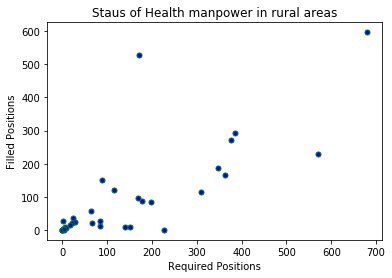
\includegraphics[ scale=0.7]{images/scatter_plot.png}
\caption{Scatter plot for the health manpower}
\label{visina8}
\end{center}
\end{figure}

\begin{figure}[h!]
\begin{center}
\advance\leftskip-2cm
\advance\rightskip-2cm
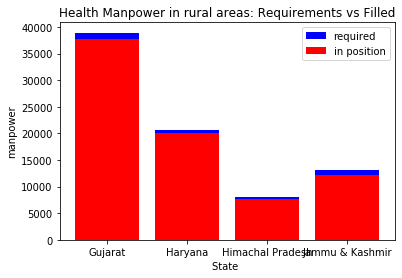
\includegraphics[ scale=0.7]{images/bar_plot.png}
\caption{Bar plot for the health manpower}
\label{visina8}
\end{center}
\end{figure}

\begin{figure}[h!]
\begin{center}
\advance\leftskip-2cm
\advance\rightskip-2cm
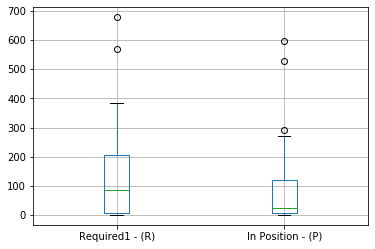
\includegraphics[ scale=0.7]{images/box_plot.png}
\caption{Box plot for the health manpower}
\label{visina8}
\end{center}
\end{figure}


\bibliographystyle{IEEEtran}
\bibliography{question_03.bib}

\end{document}
